\documentclass[a4paper, 10pt]{report}
\usepackage[italian]{babel}
\usepackage[T1]{fontenc}
\usepackage[utf8]{inputenc}
\usepackage{charter}
\usepackage{amsmath}
\usepackage{amsthm}
\usepackage{amsfonts}
\usepackage{graphicx}
\usepackage{wrapfig}
\usepackage{tcolorbox}
\usepackage{fancyhdr}
\usepackage{listings}
\usepackage{longtable}
\usepackage{multicol}
\usepackage{xcolor}

\usepackage{geometry}
\geometry{a4paper, left=2cm,right=2cm,top=2cm,bottom=2cm}

\pagestyle{fancy}
\lhead{}
\chead{}
\rhead{\bfseries 17 ottobre 2019 }
\lhead{\bfseries Segnali e immagini - laboratorio}

\newcounter{main}
\setcounter{main}{1}

\lstnewenvironment{code}[1][firstnumber=\themain,name=main]
  {\lstset{language=matlab,
           basicstyle=\medium\ttfamily,
           numbers=left,
           basicstyle=\small,
           columns=fullflexible,
           #1
          }
}
{\setcounter{main}{\value{lstnumber}}}


\begin{document}

\noindent \textbf{Esempio di Cross correlazione tra segnali di vibrazione:}

\begin{code}
load noisysignals s1 s2;  % caricamento segnali

[acor,lag] = xcorr(s2,s1);
[~,I] = max(abs(acor));  %estraggo l'indice associato al valore assoluto massimo in acor
timeDiff = lag(I);   %estraggo lo shift relativo al valore di cross - correlazione massimo
      
figure;

subplot(411); plot(s1); title('s1');
subplot(412); plot(s2); title('s2');
subplot(413); plot(lag,acor);

subplot(414); plot([zeros(1,-timeDiff) s2']);
hold on; plot(s1);
title('Cross-correlation between s1 and s2')
\end{code}

\noindent \\Analisi codice:
\begin{longtable}{| p{.20\textwidth} | p{.75\textwidth} |}

\textbf{max(X)} & Ritorna il valore massimo nell'array X.
\\\\
\textbf{[val, i] = max(X)} & Assegna il valore massimo dell'array X a val e a i il realtivo indice.
\\

\end{longtable}

\noindent Osservazioni:
\begin{itemize}
\item[-] Posso usare \textasciitilde \hspace{0.1cm} in un assegnamento per dire che il valore non mi interessa (es: una funzione torna due valori e mi interessa solo il secondo. Quindi il primo lo assegno a \textasciitilde);
\item[-] Nelle righe 13 - 14 disegno il segnale s2 (lo faccio partire da timeDiff per rappresentare la cross correlazione nel punto maggiore) e ci sovrappongo s1.
\end{itemize}

\noindent Risultato:
\begin{center}
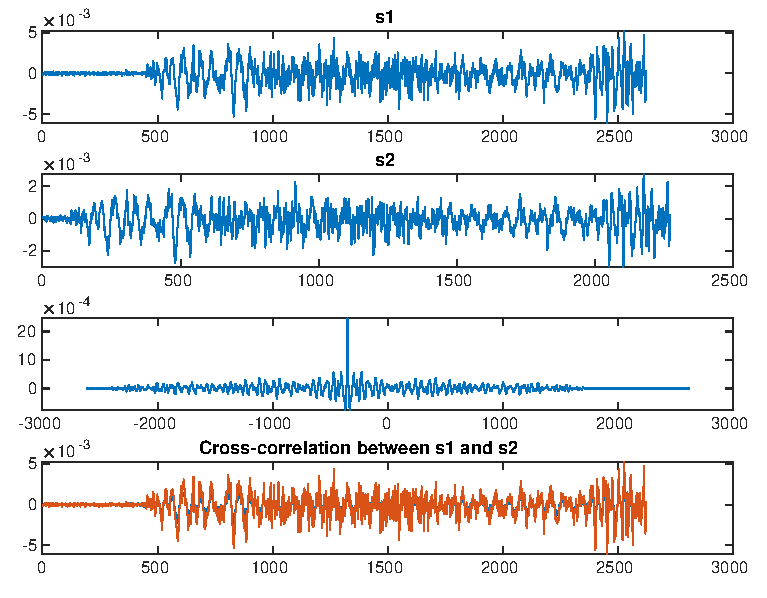
\includegraphics[scale=1]{es3.pdf}
\end{center}















\end{document}